\chapter{Campagna sperimentale}
Nota bene viene usat lo stesso seed per il training, in questo si generarno gli sessi folds
s
\section{Approccio}
\subsection{10-folds cross validation}
Per la fase di training dei modelli viene utilizzata la tecnica k-folds cross validation. Si procede quindi creando una partizione del dataset iniziale, dove ogni sottoinsieme, ovvero un fold, ha circa lo stesso numero di istanze ed è più o meno bilanciato tra la classe positiva e negativa.

Per gli esperimenti effettuati, è stato scelto $k = 10$, ovvero il dataset viene diviso casualemnte in 10 parti, utilizzando ad ogni iterazioni una porzione di dati diversa per il trainig-set e test-set. Avendo scelto questo valore di k, la proporzione tra i due insiemi sarà sempre 90\% per il training-set e 10\% per il test-set.

Per ogni modello si vogliono testare diversi iperparametri (\autoref{sec:mode_selection}), pertanto ad ogni iterazione della 10-folds, fissato un fold per il training $\hat{F}$, si esegue un'altra 10-fold cross validation più interna su $\hat{F}$  ($90\%$ del dataset totale), così da poter scegliere l'iperparametro migliore.

Procedendo in questo modo l'ottimizzazione degli iperparametri viene effettuata sfruttando solo il training set e il test set non viene utilizzato nè per il training nè per la scelta degli iperparametri ottimali.

\begin{figure}[H]
	\centering
	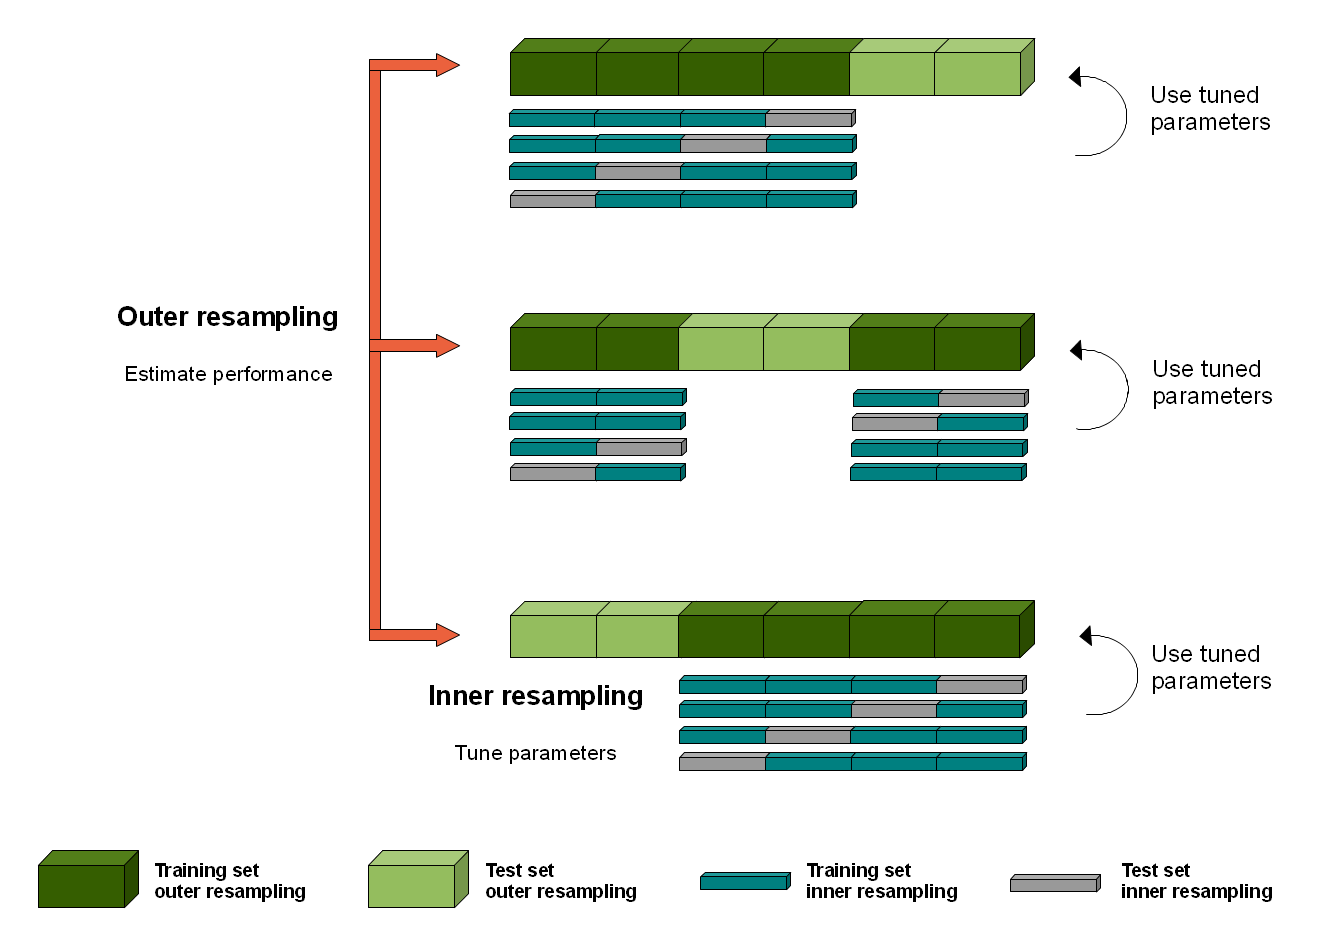
\includegraphics[width=13cm]{assets/nested-cv.png}
	\caption{Nested 3-folds cross validation.}
\end{figure}

Una nota importante è che i 10 folds vengono generati in modo casuale, tuttavia per ogni modello di cui si vuole fare il training, questa generazione casuale viene effettuata a partire dallo stesso seed. Questo garatisce di avere folds generati casualmente ma in modo idenctico per ogni modello, in questo modo si ottengono dei risultati statisticamente validi.

\subsection{Model selection}
\label{sec:mode_selection}

\subsubsection{Grid search}
\label{sec:grid-search}
Hyperparameter optimization


\section{Misure di performance}
\subsection{Accuracy}
\subsection{Precision, Recall e F-measure}
\subsection{Curve ROC}

\section{Support Vector Machine}
\subsection{Kernel}

\section{Decision Tree} \subsection{Scelta del modello} Come secondo
modello parte del progetto é stato scelto un albero di decisione
(decision tree/classification tree). Questo perché anche con un
dataset relativamente ampio permette il training in un tempo
ragionevole rispetto alla potenza computazionale in nostro possesso.

\section{Esperimenti}
\subsection{Performance}
\section{Modelli a confronto}
